\chapter{Guía de instalación}

\section{Requerimientos}
Previo a la instalación del paquete, el usuario debe cerciorarse de que su 
equipo de cómputo cumpla con los siguiente:

\begin{itemize}
 \item MATLAB 2015b o superior debe estar instalado en el sistema de cómputo del 
usuario.

% \begin{itemize}
%  \item El equipo de cómputo debe cumplir también con los requerimientos especificados
% por MATLAB.
% \end{itemize}
 \item Espacio disponible en disco de 10 MiB o superior.
 \item [\textbf{Opcional}] Contar con un reproductor de videos 
instalado en su equipo de cómputo para poder reproducir los archivos MP4 
generados por el programa.
% \item [\textbf{Opcional}] Contar con una interfaz funcional de Git instalada. 
% Este requerimiento es exclusivo para usuarios que deseen clonar el repositorio.
\end{itemize}


\section{Descarga del software y actualizaciones}
La versión más reciente del simlador GSP se encuentra disponible en 
\href{https://github.com/der-coder/cinvestav-robotics-project/tree/master}{GitHub} 
\footnote{https://github.com/der-coder/cinvestav-robotics-project}. El usuario es
libre de descargar el software como un comprimido zip o clonar el repositorio de 
acuerdo a sus necesidades. La instalación del paquete es la misma para ambos casos
posterior a la descarga y descompresión de los archivos.

Una copia de la versión estable más reciente del simulador se incluye en la memoria
técnica del proyecto. Su instalación sigue el mismo proceso que los métodos de descarga
descritos anteriormente.

\subsection{Archivo zip}
La descarga del comprimido se realiza desde la página del proyecto, como se muestra 
en la figura \ref{fig: descarga zip}. El usuario puede hacer uso de cualquier programa 
de descompresión, como \href{https://www.7-zip.org/}{7-Zip}\footnote{https://www.7-zip.org/}, 
para extraer su contenido una vez concluida su descarga.

\begin{figure}[h]
 \centering
 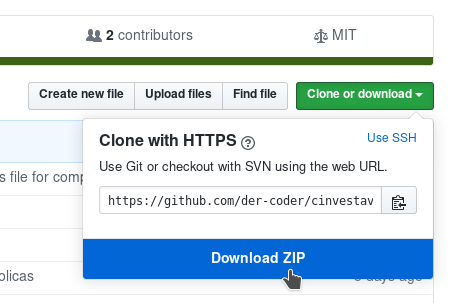
\includegraphics{img/install_github_download_zip.png}
 % install_github_download_zip.png: 472x303 px, 96dpi, 12.49x8.02 cm, bb=0 0 354 227
 \caption{Descarga del paquete en formato comprimido zip.}
 \label{fig: descarga zip}
\end{figure}

% \subsection{Clonar el repositorio}
% 
% Los usuarios que deseen mantenerse al tanto de las actualizaciones más recientes
% pueden clonar el repositorio en vez de descargar el comprimido zip desde el mismo 
% portal web. Se recomienda navegar hasta el directorio en el que el usuario trabajará
% a manera de facilitar la detección del código por parte de MATLAB.
% 
% El proceso de clonado en \emph{Windows} se realiza a través de la interfaz gráfica 
% que el usuario haya instalado. Para los sistemas operativos \emph{GNU/Linux} y 
% \emph{Mac OS} se puede realizar a través de la terminal con el siguiente comando:
% 
% 
% \begin{center}
% \begin{lstlisting}[language=bash, frame=single]
% $ git clone <URL del repositorio> 
% \end{lstlisting}
% \end{center}
% 
% Para actualizar el código, basta emitir en la terminal el siguiente comando
% 
% \begin{center}
% \begin{lstlisting}[language=bash, frame=single]
% $ git pull
% \end{lstlisting}
% \end{center}

\section{Instalación}

Es posible instalar de dos maneras el simulador: inclusión en el 
directorio de trabajo o la inclusión del código en 
la variable \emph{MATLABPATH} de MATLAB. El primer método no requiere acceso
administrativo a las carpetas del sistema y se detalla a continuación.

\begin{enumerate}
 \item Copiar o cortar la carpeta que contiene el código del simulador.
 \item Navegar al directorio de trabajo desde el explorador de archivos.
 \item Depositar el la carpeta en el directorio
\end{enumerate}

MATLAB es capaz de detectar automáticamente todos los archivos del simulador en 
el ambiente de trabajo actual si se encuentran en la carpeta de trabajo.

Para el segundo método, basta agregar la dirección en la que se encuentra la 
carpeta a la variable \emph{MATLABPATH} en el sistema. 

\begin{itemize}
 \item [Windows] Se realiza desde \textbf{Panel de Control}, \textbf{Sistema},
 \textbf{Ajustes avanzados de sistema}, \textbf{Variables de Entorno}.
 \item [Mac, Linux] Exportar el valor de \emph{MATLABPATH} desde la terminal.
\end{itemize}


 

%  Reference for Toolbox installation 
%  https://www.mathworks.com/help/matlab/ref/matlab.addons.toolbox.installtoolbox.html
